\documentclass[11pt,a4paper]{article}
\usepackage[utf8]{inputenc}
\usepackage[T1]{fontenc}
\usepackage{amsfonts}
\usepackage[french]{babel}
\frenchbsetup{StandardLists=true} % à inclure si on utilise \usepackage[francais]{babel}
\usepackage{enumitem}
\usepackage{amssymb}
\usepackage{amsmath}
\usepackage[left=2cm,right=2cm,top=2cm,bottom=2cm]{geometry}
\usepackage{multirow}
\usepackage[dvipsnames]{xcolor}

\usepackage[T1]{fontenc}
\usepackage{fouriernc}
\usepackage{graphicx}

%\usepackage{setspace}
%\singlespacing

\usepackage{pstricks}
\usepackage{xkeyval}
\usepackage{pst-labo}


\usepackage{multicol}
\setlength{\columnsep}{1cm}
\usepackage{caption}
\usepackage{fancyhdr}
\pagestyle{fancy}
\renewcommand\headrulewidth{1pt}
\fancyhead[L]{Lycée Denis Diderot }
\fancyhead[R]{Classe de 1 Bac Pro }
\setcounter{page}{1}\fancyfoot[C]{page \thepage}
\fancyfoot[R]{Année 2025-2026}
\fancyfoot[L]{Alexis RUIZ}
\usepackage{multirow,tabularx,booktabs}
\usepackage[tikz]{bclogo} 
\usepackage{qrcode}

\newcommand{\cadreblanc}[1]{%
\medskip\framebox[\linewidth][c]{%
\rule{0mm}{#1mm}}\par
\medskip}

\usepackage{colortbl}
\usepackage{awesomebox}
\setlength{\aweboxvskip}{0mm}
\usepackage{pifont}
\usepackage{chemmacros}
\chemsetup{modules=all}
\setlength{\columnseprule}{.25mm}

\renewcommand{\arraystretch}{1.5}
\newcommand*\acocher{\quitvmode{\fboxsep0pt \fboxrule0.8pt \fbox{\vrule height1.8ex depth.1ex width0pt \vrule height0pt depth0pt width1.9ex }}}

\newcolumntype{C}[1]{>{\centering\arraybackslash }b{#1}}

\newcommand{\code}{\awesomebox[black]{2pt}{

\includegraphics[scale=0.15]{../Chapitre 1 - Energie et puissance électrique/images/frame.png}
}{black}}

\newcommand{\moteur}{\awesomebox[black]{2pt}{

\includegraphics[scale=1]{images/moteur.jpg} 
}{black}}

\newcommand{\defconclusion}{\awesomebox[black]{2pt}{\rotatebox{90}{\Large{\textbf{Conclusion}}}}{black}}

\newcommand{\defbox}{\awesomebox[black]{2pt}{
\includegraphics[scale=0.5]{../Chapitre 1 - Energie et puissance électrique/images/appel exam.png}}{black}}

  \newenvironment{itemize*}%  % listes compactes
    {\begin{itemize}%
      \setlength{\itemsep}{0pt}%
      \setlength{\parskip}{0pt}}%
    {\end{itemize}}

\frenchbsetup{StandardLists=true}



\begin{document}

\flushleft \textbf{NOM : \hfill Classe : \hspace{3cm} ~~\\[2mm]
Prénom:\\[0,4cm]
}
\hrule\
%\\[0,1cm]

\begin{center}
 \LARGE{TP1  - Étude d'un mouvement rectiligne uniforme  }
\end{center}

%\vspace{2 mm}

\normalsize

\hrule\
\\[0,2cm]
   \begin{center}
   \textbf{Le soin et la rédaction interviendront dans la notation.}
   \end{center} 

\noindent%
\begin{minipage}{.4\textwidth}%

    
 \begin{bclogo}[couleur=white ,  arrondi =0.1 , logo = \bcinfo, epBarre =2]{ Matériel }

\begin{itemize*}
    \item 1 calculatrice Ti83 CE
    \item 1 Ti Rover
    \item 1 smartphone
    \item 1 règle d'1m

\end{itemize*}
\end{bclogo}

\end{minipage}%
\hspace{2cm}
\begin{minipage}{.25\textwidth}%
\begin{center}
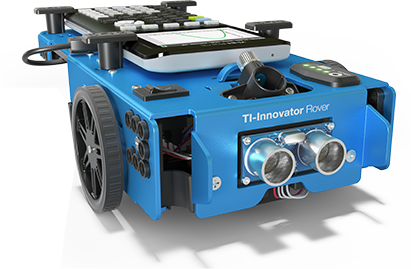
\includegraphics[width=\textwidth]{images/TiROVER.png}
\end{center}
\end{minipage}%

\vfill 


\fcolorbox{black}{white}{\textbf{Protocole}}

\begin{itemize}
    \begin{multicols}{2}
    \item Positionner l'écran en bout de table côté mur. 
    
    \item Positionner le Rover à droite de la table. 
    
    \item Allumer la calculatrice.
    
    \item Aller dans \fbox{prgm} puis choisir \texttt{1:Ti-Basic}.

    \item Choisir le programme \texttt{ROVER3}.

    \item Lancer le programme.

    \item Décrire la trajectoire du Rover : 

    \cadreblanc{15}

    \item Recommencer le processus en filmant avec votre téléphone. 

    \end{multicols}

    \item Télécharger l'application Fizziq sur votre téléphone. \hfill 
\noindent%
\begin{minipage}{.2\textwidth}%

~~Android : \\[3pt]
\qrcode{https://play.google.com/store/apps/details?id=com.chazot.fizziq&hl=fr}
\end{minipage}%
\hfill 
\begin{minipage}{.20\textwidth}%
\begin{center}
~~IPhone : \\[3pt]
\qrcode{https://apps.apple.com/fr/app/fizziq/id1516870599}
\end{center}
\end{minipage}%

\vfill 

\fcolorbox{black}{white}{\textbf{Mesures}} Ouvrir l'application Fizziq puis choisir pour importer votre vidéo : \\[2mm]


\noindent%
\begin{minipage}{.2\textwidth}%
\begin{center}
Analyse\\cinématique 
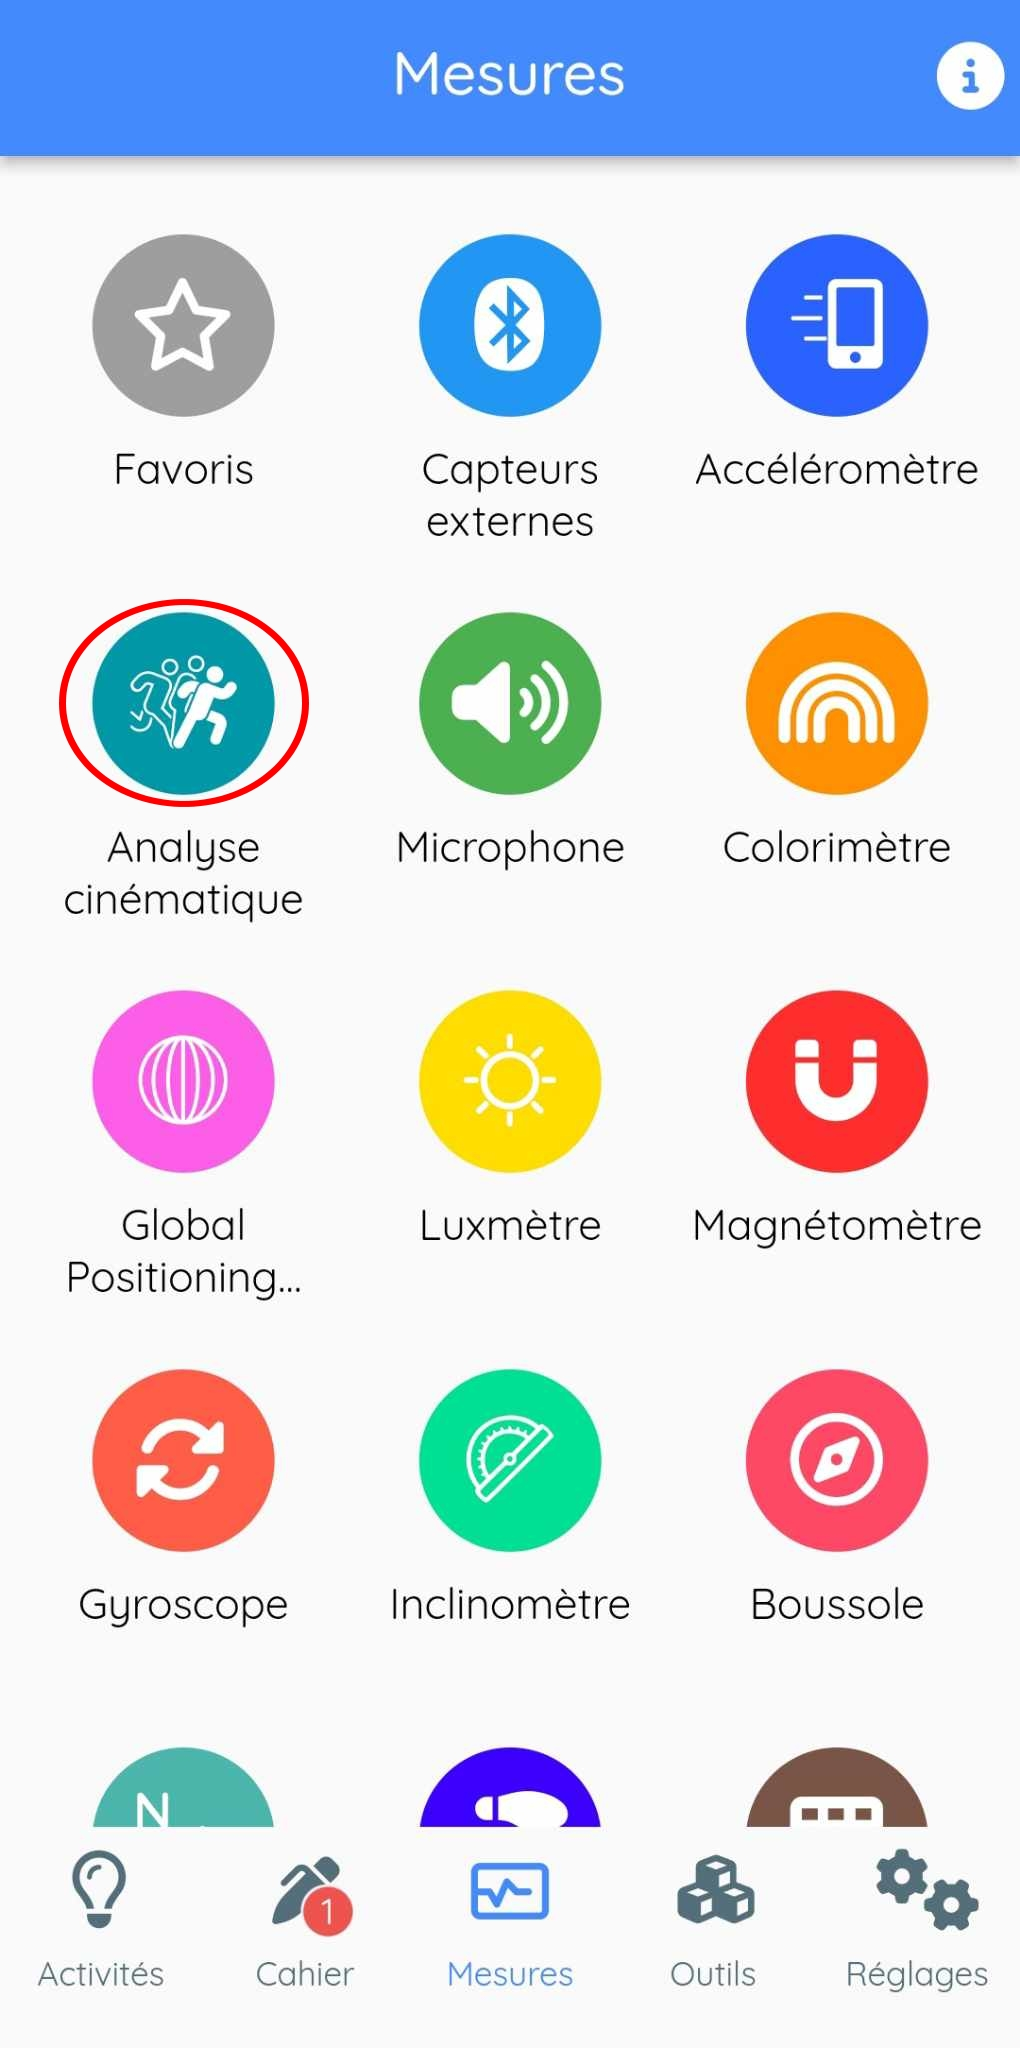
\includegraphics[width=\textwidth]{images/1.jpg}
\end{center}
\end{minipage}%
\hfill
\begin{minipage}{.2\textwidth}%
\begin{center}
Cinématique \\par vidéo 
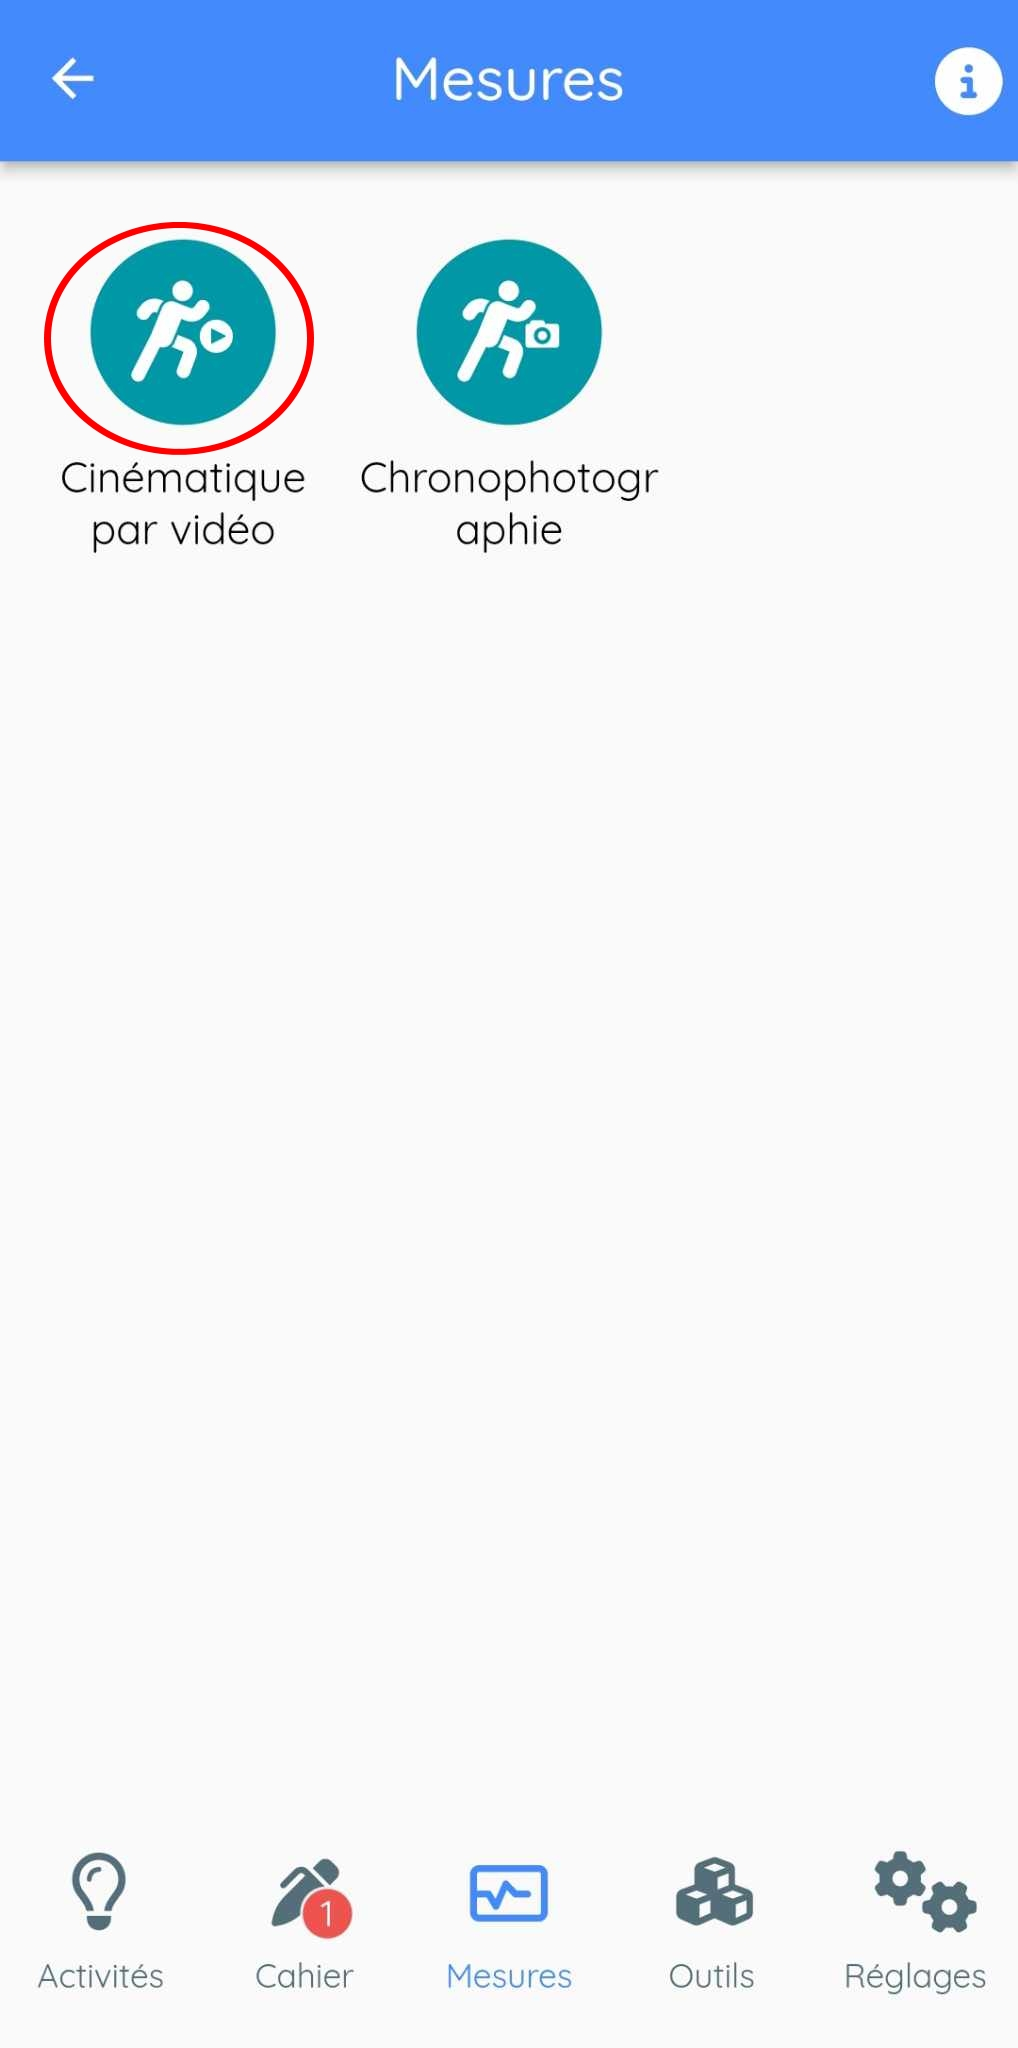
\includegraphics[width=\textwidth]{images/2.jpg}
\end{center}
\end{minipage}%
\hfill
\begin{minipage}{.20\textwidth}%
\begin{center}
Mes vidéos
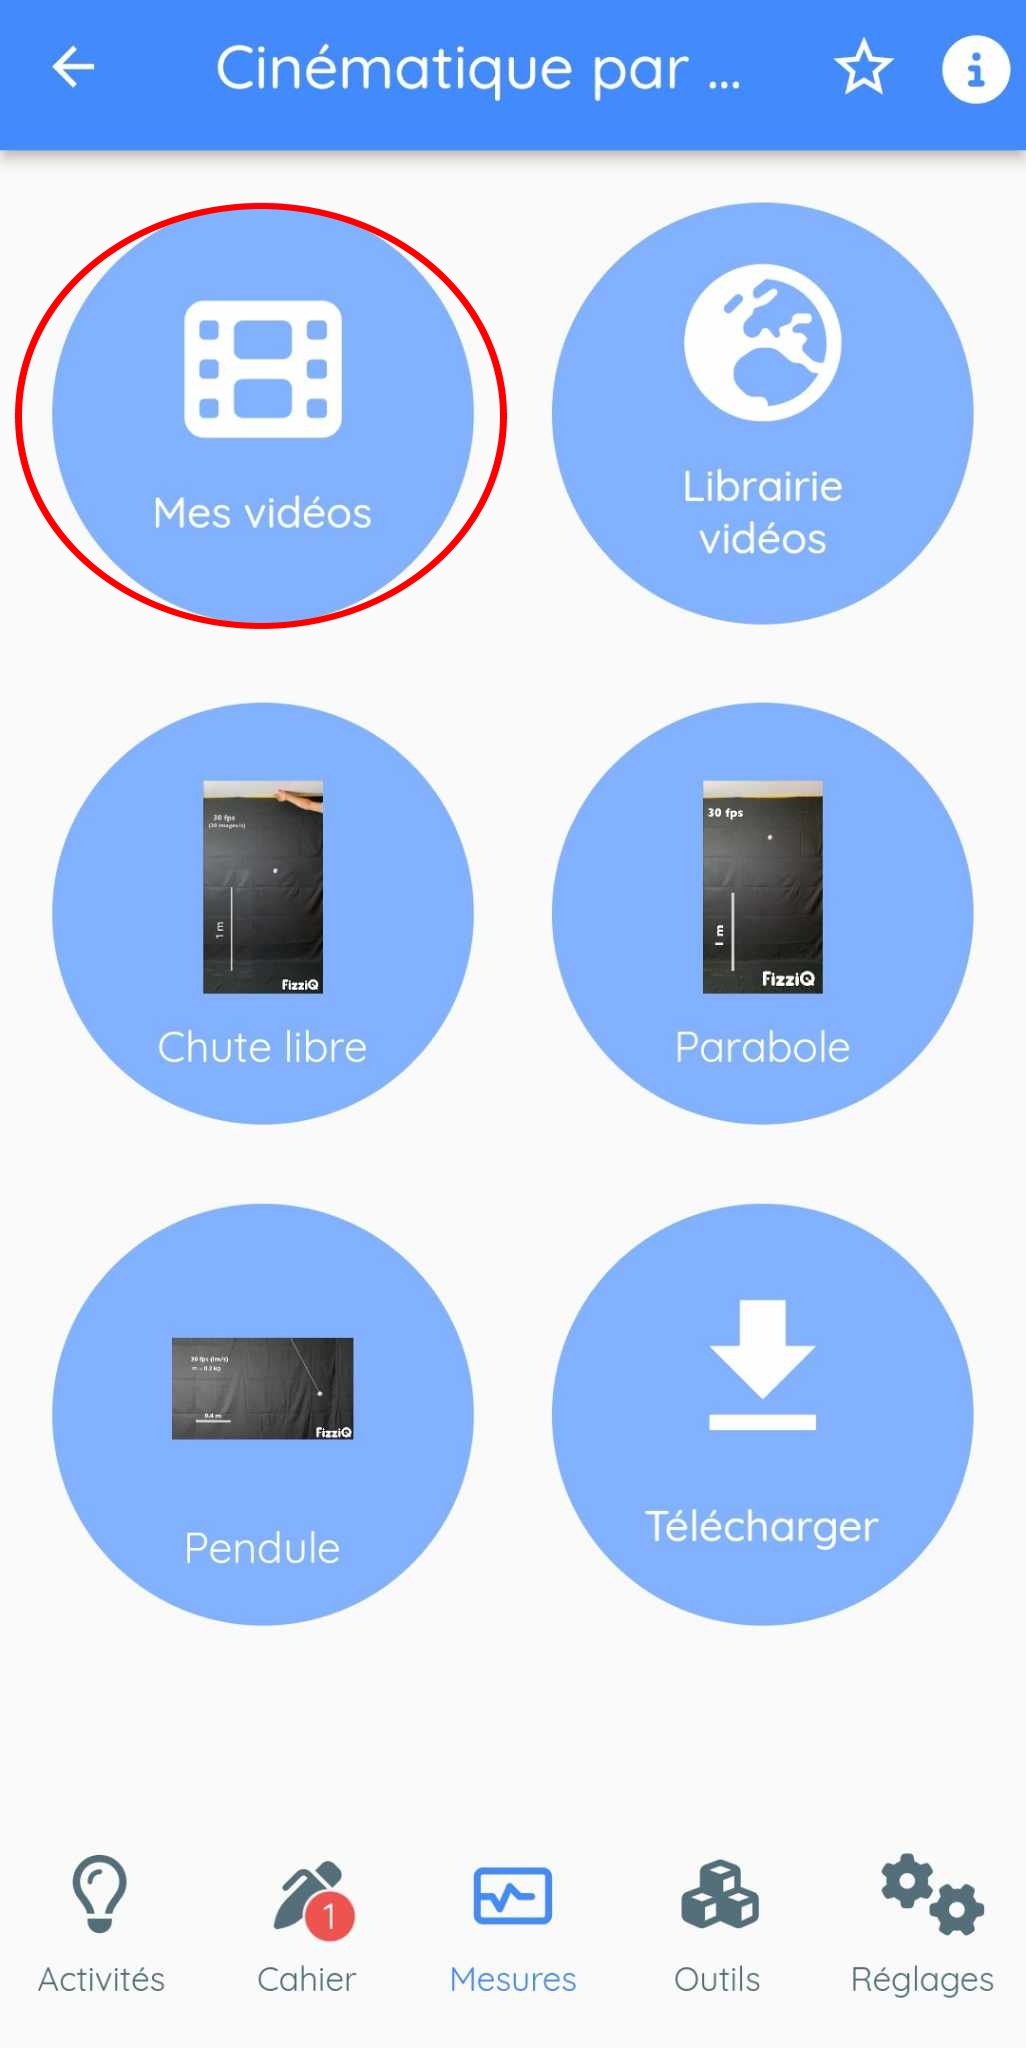
\includegraphics[width=\textwidth]{images/3.jpg}
\end{center}
\end{minipage}%


\vfill  

    \newpage

    \begin{multicols}{2}


\item Réglage de la longueur de la règle : \\[5mm]
\begin{itemize}
    \item Sur la nouvelle fenêtre, positionner l'origine du repère sur le 0 , puis l'extrémité sur 1m.
    \item Préciser dans la fenêtre en haut à gauche la longueur de la règle en mètre (m)

\end{itemize}

\begin{center}
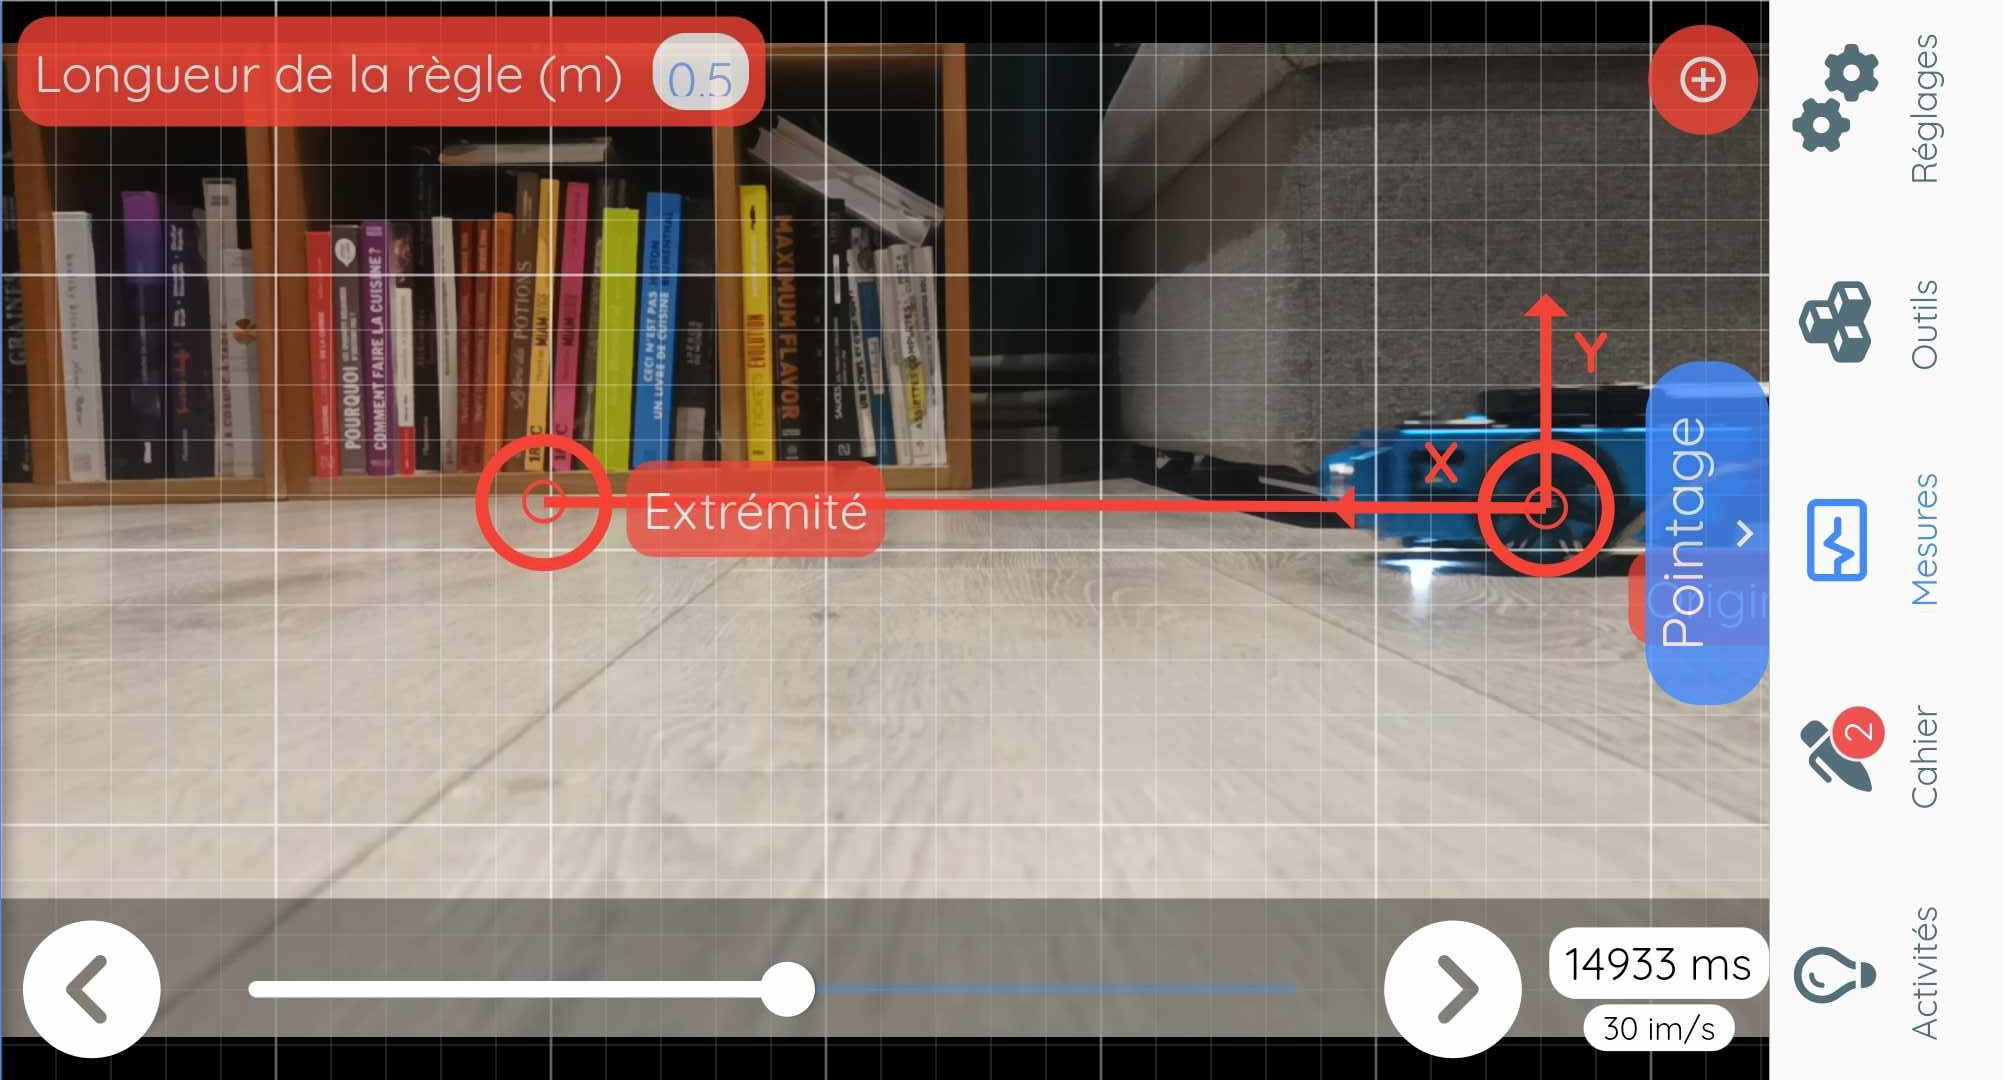
\includegraphics[scale=0.11]{images/4.jpg}
\end{center}

\columnbreak

\item Sélectionner Pointage : 
\begin{itemize}
    \item Régler l'intervalle de temps $\mathrm{\Delta t ~à~200 ms}$
    \item Positionner la mire au centre de la roue et cliquer. 
    \item La vidéo passe alors à l'image suivante. Recommencer l'opération pour obtenir 10 valeurs.  
\end{itemize}
\begin{center}
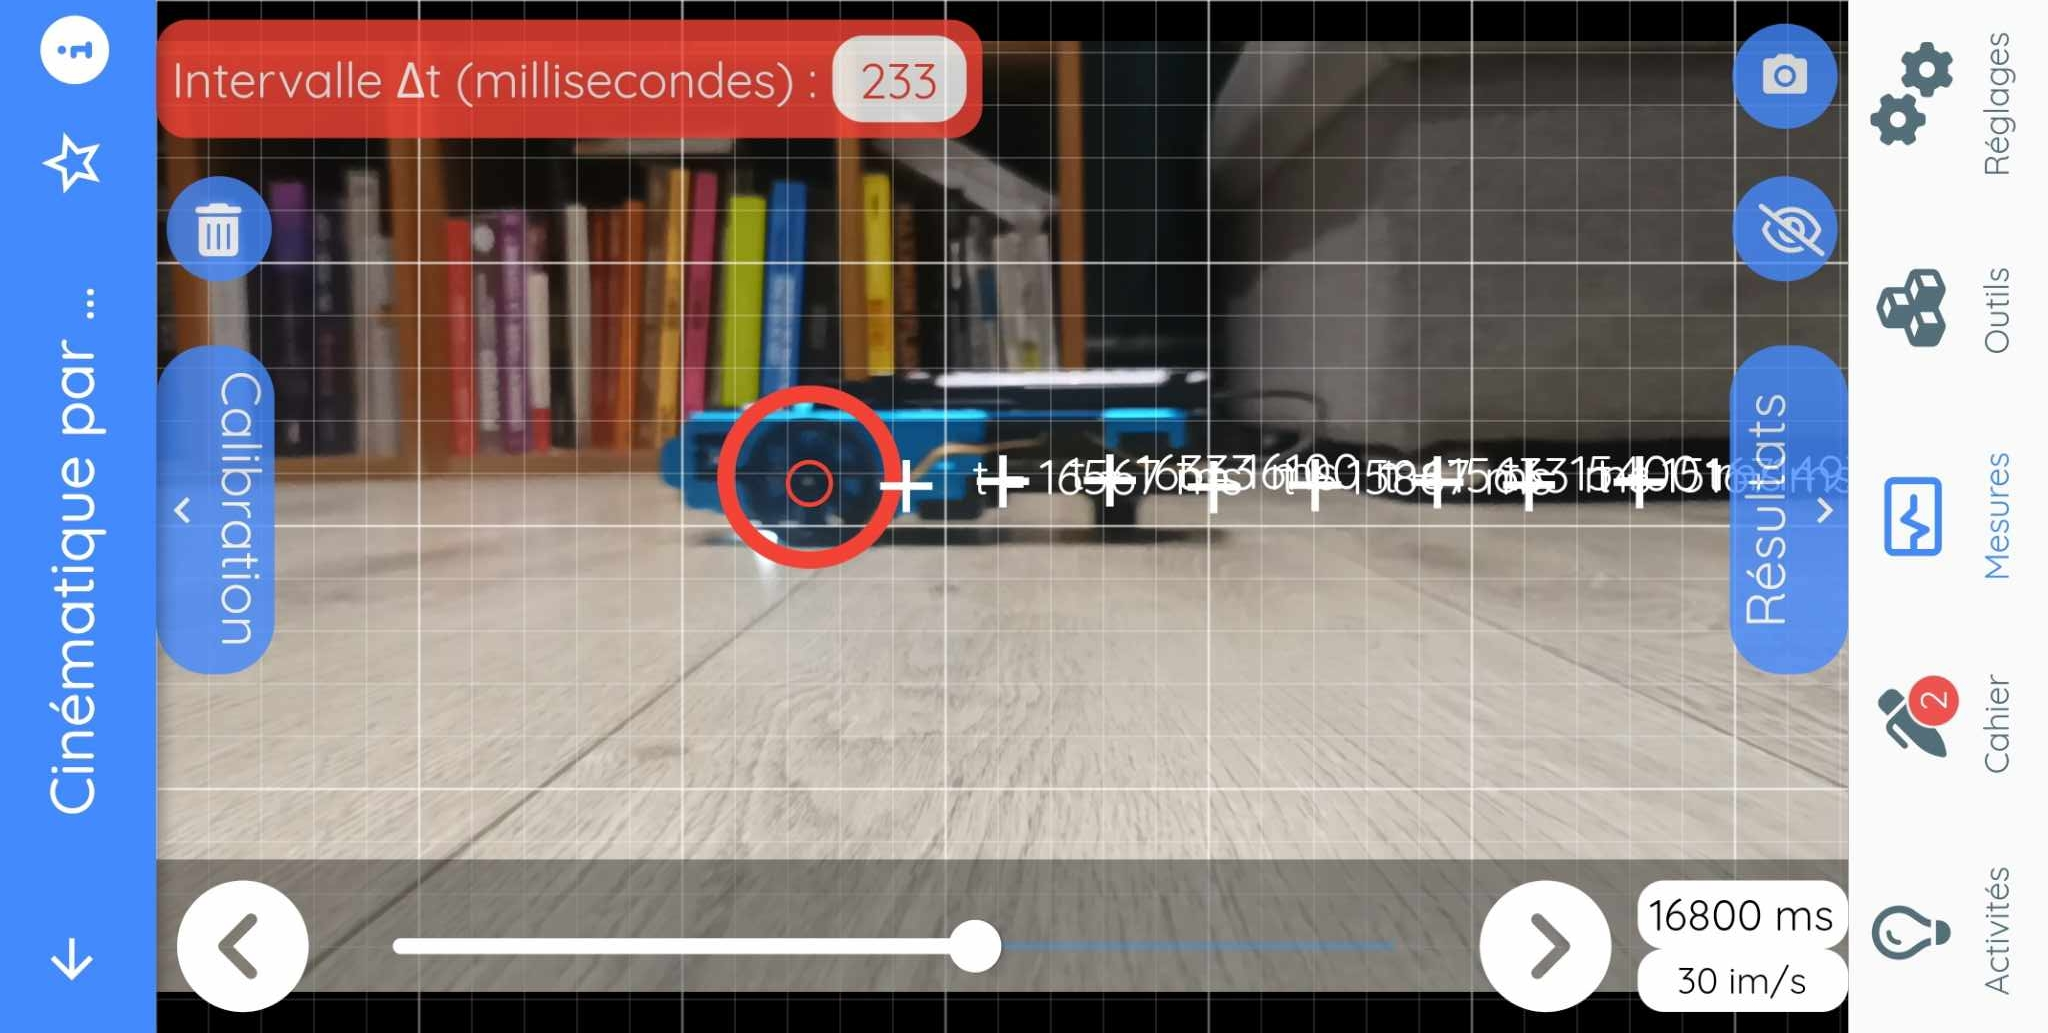
\includegraphics[scale=0.11]{images/5.jpg}
\end{center}

\end{multicols}

\end{itemize}





\fcolorbox{black}{white}{\textbf{Mesures}}\\
\ding{202} Aller dans Mesures, cocher T(s), le temps en secondes et x(m), la distance en mètre. \\Compléter le tableau suivant : 

\begin{center}
    
\renewcommand{\arraystretch}{2}
    \begin{tabular}{|C{3cm}||C{0.8cm}|C{0.8cm}|C{0.8cm}|C{0.8cm}|C{0.8cm}|C{0.8cm}|C{0.8cm}|C{0.8cm}|C{0.8cm}|C{0.8cm}|}
         \hline
         Point ($i$) & 1 &  2& 3 & 4 & 5 & 6& 7& 8& 9 & 10\\
         \hline
         $t_i(s)$ &  &  &  &  &  & & & & & \\
         \hline
          $x_i(m)$ &  &  &  & & & & & & & \\
         \hline
 
    \end{tabular}



\begin{minipage}{0.9\textwidth}%

    

 
 \begin{bclogo}[couleur=white ,  arrondi =0.1 , logo = \bcinfo, epBarre =2]{ MÉTHODE : Calcul de la vitesse $v_i$}
\begin{center}
    

 Pour la calculer la vitesse instantanée au point $i$, on calcule la vitesse entre les points $i-1$ et $i+1$. \\[1cm]
 

 Ce qui nous donne : $v_i=\dfrac{x_{i+1}-x_{i-1}}{t_{i+1}-t_{i-1}}$   
\hspace{2cm}
 Exemple pour $i=1$ , $v_2=\dfrac{x_{2}-x_{0}}{t_{2}-t_{0}}$ \\[1cm]

\textbf{ Remarque : en utilisant cette méthode , on ne peut calculer $v_0$ et $v_{10}$}

 \end{center}
\end{bclogo}

\end{minipage}

\vfill 

\end{center}

\ding{203} Compléter le tableau suivant : 
\begin{center}
    
\renewcommand{\arraystretch}{2}
    \begin{tabular}{|C{3cm}||C{0.8cm}|C{0.8cm}|C{0.8cm}|C{0.8cm}|C{0.8cm}|C{0.8cm}|C{0.8cm}|C{0.8cm}|C{0.8cm}|C{0.8cm}|}
         \hline
         Point ($i$) & 1 &  2& 3 & 4 & 5 & 6& 7& 8& 9 & 10\\
         \hline
         $t_{i+1}-t_{i-1}$ &  &  &  &  &  & & & & & \\
         \hline
          $x_{i+1}-x_{i-1}$ &  &  &  & & & & & & & \\
           \hline
          $v_i(m/s)$ & \cellcolor{gray!30} &  &  & & & & & & & \cellcolor{gray!30}\\
         \hline
 
    \end{tabular}


\end{center}

\newpage

\ding{204} Compléter le graphique en utilisant les valeurs du tableau. On prendra $t_1$ comme origine des temps sur l'axe des abscisses. 


\begin{center}
    
\begin{tikzpicture}[scale=1]
%papier milli
\draw [very thin, gray!20] (0,-3) grid[step=0.1] (11,8);

\draw [very thin, black!20] (0,-3) grid[step=0.5] (11,8);
\draw [very thin, black!40] (0,-3) grid[step=1] (11,8);
\draw[->,>=stealth] (0,-3) -- (11.5,-3) node[below right] {$t_i(s)$};
%stealth définit un style de flèche, "furtif"
\draw[->,>=stealth] (0,-3) -- (0,8.2)node[below left] {$x_i$};

\draw (0,-2.9) -- (0,-3.1) node [below right] {{\scriptsize $t_1$}}; 

\draw (0,-3) -- (-0.10,-3) node [left] {{\scriptsize $0$}}; 

%\draw (3,-2.9) -- (3,-3.1) node [below left] {{\scriptsize 60}}; %échelle abscisse
%\draw (0.1,-1) -- (-0.1,-1) node [left] {{\scriptsize 1000}}; %échelle ordonnée

\end{tikzpicture}
\end{center}

\vspace{1cm}



\fcolorbox{black}{white}{\textbf{Interprétation }} \\[5mm]
\ding{205} Commentez la représentation graphique que vous avez obtenue. \\



\cadreblanc{25}

\vspace{1cm}

\ding{206} Comparer les valeurs de la vitesse : 
\vspace{3mm}
\dotfill

\vspace{1cm}

\ding{207} La vitesse : \hspace{5mm} $\square$~augmente \hspace{3cm} $\square$~reste constante\hspace{3cm} $\square$~diminue


\vfill 








\end{document}